\documentclass{beamer}
\usecolortheme{dove}
\setbeamertemplate{navigation symbols}{}
\usepackage{amsmath,amssymb,amsfonts,amsthm, multicol, subfigure, color}



\usepackage{bm}
\usepackage{graphicx}
\usepackage{tabularx}
\usepackage{booktabs}
\usepackage{hyperref}
\usepackage{pdfpages}
\def\independenT#1#2{\mathrel{\rlap{$#1#2$}\mkern2mu{#1#2}}}
\newcommand\indep{\protect\mathpalette{\protect\independenT}{\perp}}
\def\log{\text{log}}
\newcommand\logit{\text{logit}}
\newcommand\iid{\stackrel{\text{iid}}{\sim}}
\newcommand\E{\text{E}}
\newcommand\V{\text{V}}
\renewcommand\P{\text{P}}
\newcommand{\Cov}{\text{Cov}}
\newcommand{\Cor}{\text{Cor}}
\newcommand\doop{\text{do}}


\usepackage{stackrel}
\usepackage{tikz}
\usetikzlibrary{arrows,shapes.arrows,positioning,shapes,patterns,calc}
\newcommand\slideref[1]{\vskip .1cm \tiny \textcolor{gray}{{#1}}}
\newcommand\red[1]{\color{red}#1}
\newcommand\blue[1]{\color{blue}#1}
\newcommand\gray[1]{\color{gray}#1}
\newcommand\seagreen[1]{\color{seagreen}#1}
\newcommand\purple[1]{\color{purple}#1}
\newcommand\orange[1]{\color{orange}#1}
\newcommand\black[1]{\color{black}#1}
\newcommand\white[1]{\color{white}#1}
\newcommand\teal[1]{\color{teal}#1}
\newcommand\magenta[1]{\color{magenta}#1}
\newcommand\Fuchsia[1]{\color{Fuchsia}#1}
\newcommand\BlueGreen[1]{\color{BlueGreen}#1}
\newcommand\bblue[1]{\textcolor{blue}{\textbf{#1}}}
\newcommand\bred[1]{\textcolor{red}{\textbf{#1}}}
\newcommand\bgray[1]{\textcolor{gray}{\textbf{#1}}}
\newcommand\bgreen[1]{\textcolor{seagreen}{\textbf{#1}}}
\newcommand\bref[2]{\href{#1}{\color{blue}{#2}}}
\colorlet{lightgray}{gray!40}
\pgfdeclarelayer{bg}    % declare background layer for tikz
\pgfsetlayers{bg,main} % order layers for tikz
\newcommand\mycite[1]{\begin{scriptsize}\textcolor{darkgray}{(#1)}\end{scriptsize}}
\newcommand{\tcframe}{\frame{
%\small{
\only<1|handout:0>{\tableofcontents}
\only<2|handout:1>{\tableofcontents[currentsection]}}
%}
}

\setbeamertemplate{footline}[frame number]

\setbeamertemplate{navigation symbols}{}

\addtobeamertemplate{footline}{
	\leavevmode%
	\hbox{%
		\begin{beamercolorbox}[wd=\paperwidth,ht=2.75ex,dp=.5ex,right,rightskip=1em]{mycolor}%
			\usebeamercolor[fg]{navigation symbols}\insertslidenavigationsymbol%
		\end{beamercolorbox}%
	}%
	\vskip0.5pt%
}{}





\usepackage[round]{natbib}
\bibliographystyle{humannat-mod}
\setbeamertemplate{enumerate items}[default]
\usepackage{mathtools}

\newcommand{\goalsframe}{\begin{frame}{Learning goals for today}
At the end of class, you will be able to:
\begin{enumerate}
\item Identify a sufficient adjustment set for the backdoor criterion
\item Assess whether selection bias may hold in a gathered sample
\end{enumerate} \vskip .2in
\end{frame}}

\title{Discussion}
\author{INFO/STSCI/ILRST 3900: Causal Inference}
\date{20 Sep 2023}

\begin{document}

\begin{frame}[noframenumbering,plain]
  \titlepage
\end{frame}




\begin{frame}
\frametitle{Open or blocked?}

How to check if a path is open or blocked:
\begin{enumerate}
    \item Traverse the path node by node 
    \item If any node is blocked, the entire path is blocked
    \item If all nodes are open, then entire path is open
\end{enumerate}

\vspace{2em}

How to check if a node is open or blocked:
\begin{itemize}
    \item If non-collider:
    \begin{itemize}
        \item Open if it is not in the conditioning set
        \item Blocked if it is in the conditioning set
    \end{itemize}
    \item If collider:
    \begin{itemize}
        \item Open if it or any of its descendants are in the conditioning set
        \item Otherwise it is blocked
    \end{itemize}
\end{itemize}

\end{frame}


\begin{frame}
\frametitle{Practice}

  \begin{figure}[t]
\begin{tikzpicture}[x = \textwidth, y = .5\textheight]
\node (A) at (.2, .5) {A};
\node (Z) at (.5, .5) {Z};
\node (Y) at (.8, .5) {Y};
\node (H) at (.65, .7) {H};

\draw[->, thick] (A) -- (Z);
\draw[->, thick] (H) -- (Z);
\draw[->, thick] (H) -- (Y);
\draw[->, thick] (Z) -- (Y);
\draw[->, thick] (H) -- (A);


\end{tikzpicture}
\end{figure}

\begin{itemize}
    \item What are the paths from $A$ to $Y$?
    \item Determine if each of the paths is causal or non-causal
    \item Determine whether each node on each path is a collider or non-collider
\end{itemize}


\end{frame}

\begin{frame}
\frametitle{Practice}

  \begin{figure}[t]
\begin{tikzpicture}[x = \textwidth, y = .5\textheight]
\node (A) at (.2, .5) {A};
\node (Z) at (.5, .5) {Z};
\node (Y) at (.8, .5) {Y};
\node (H) at (.65, .7) {H};

\draw[->, thick] (A) -- (Z);
\draw[->, thick] (H) -- (Z);
\draw[->, thick] (H) -- (Y);
\draw[->, thick] (Z) -- (Y);
\draw[->, thick] (H) -- (A);

\only<2>{
\draw[->, thick, orange] (A) -- (Z);
\draw[->, thick, orange] (Z) -- (Y);
}

\only<3>{
\draw[->, thick, orange] (H) -- (Y);
\draw[->, thick, orange] (H) -- (A);
}

\only<4>{
\draw[->, thick, orange] (A) -- (Z);
\draw[->, thick, orange] (H) -- (Z);
\draw[->, thick, orange] (H) -- (Y);
}

\only<5>{
\draw[->, thick, orange] (H) -- (Z);
\draw[->, thick, orange] (Z) -- (Y);
\draw[->, thick, orange] (H) -- (A);
}


\end{tikzpicture}
\end{figure}


\begin{itemize}
\item<only@1>
\only<2->{\item $A \rightarrow \underbrace{Z}_{\text{NC}} \rightarrow Y$ \hfill causal path}
\only<3->{\item $A \leftarrow \underbrace{H}_{\text{NC}} \rightarrow Y$ \hfill non-causal}
\only<4->{\item $A \rightarrow \underbrace{Z}_{\text{Col}}  \leftarrow \underbrace{H}_{\text{NC}} \rightarrow Y$ \hfill non-causal }
\only<5->{\item $A \leftarrow \underbrace{H}_{\text{NC}}  \rightarrow \underbrace{Z}_{\text{NC}} \rightarrow Y$ \hfill non-causal}
\end{itemize}

\end{frame}

\begin{frame}

\frametitle{Practice}
\begin{figure}[t]
\begin{tikzpicture}[x = \textwidth, y = .5\textheight]
\node (A) at (.2, .5) {A};
\node (Z) at (.5, .5) {Z};
\node (Y) at (.8, .5) {Y};
\node (H) at (.65, .7) {H};

\draw[->, thick] (A) -- (Z);
\draw[->, thick] (H) -- (Z);
\draw[->, thick] (H) -- (Y);
\draw[->, thick] (Z) -- (Y);
\draw[->, thick] (H) -- (A);


\end{tikzpicture}
\end{figure}

If we condition on $L = \emptyset$, which paths are open? Which paths are blocked?
\begin{itemize}
\item $A \rightarrow \underbrace{Z}_{\text{NC}} \rightarrow Y$ \hfill \only<2->{Open}
\item $A \leftarrow \underbrace{H}_{\text{NC}} \rightarrow Y$ \hfill \only<3->{Open}
\item $A \rightarrow \underbrace{Z}_{\text{Col}}  \leftarrow \underbrace{H}_{\text{NC}} \rightarrow Y$ \hfill \only<4->{Blocked}
\item $A \leftarrow \underbrace{H}_{\text{NC}}  \rightarrow \underbrace{Z}_{\text{NC}} \rightarrow Y$ \hfill \only<5->{Open}
\end{itemize}

\end{frame}



\begin{frame}
\frametitle{Practice}

  \begin{figure}[t]
\begin{tikzpicture}[x = \textwidth, y = .5\textheight]
\node (A) at (.2, .5) {A};
\node (Z) at (.5, .5) {\boxed{Z}};
\node (Y) at (.8, .5) {Y};
\node (H) at (.65, .7) {H};

\draw[->, thick] (A) -- (Z);
\draw[->, thick] (H) -- (Z);
\draw[->, thick] (H) -- (Y);
\draw[->, thick] (Z) -- (Y);
\draw[->, thick] (H) -- (A);


\end{tikzpicture}
\end{figure}

If we condition on $L = \{Z\}$, which paths are open? Which paths are blocked?
\begin{itemize}
\item $A \rightarrow \underbrace{\boxed{Z}}_{\text{NC}} \rightarrow Y$ \hfill \only<2->{Blocked}
\item $A \leftarrow \underbrace{H}_{\text{NC}} \rightarrow Y$ \hfill \only<3->{Open}
\item $A \rightarrow \underbrace{\boxed{Z}}_{\text{Col}}  \leftarrow \underbrace{H}_{\text{NC}} \rightarrow Y$ \hfill \only<4->{Open}
\item $A \leftarrow \underbrace{H}_{\text{NC}}  \rightarrow \underbrace{\boxed{Z}}_{\text{NC}} \rightarrow Y$ \hfill \only<5->{Blocked}
\end{itemize}

\end{frame}


\begin{frame}
\frametitle{Causal Discovery}

\begin{itemize}
    \item So far, we have assumed the DAG is known from expert knowledge
    \item DAG tells us about conditional independence we would observe in data
    \[ \text{DAG} \Rightarrow \text{Conditional independence in data} \]
    \pause
    \item Conditional independence is a observational quantity (i.e., not causal)
    \item Can be tested in observed data
    \item Can we go in the opposite direction?
    \[ \text{Conditional independence in data} \stackrel{?}{\Rightarrow} \text{DAG} \]
\end{itemize}

\end{frame}


\begin{frame}
\frametitle{Causal Discovery}

\large
Can we tell which nodes are/aren't connected by an edge?

\end{frame}


\begin{frame}
\frametitle{Causal Discovery}

  \begin{figure}[t]
\begin{tikzpicture}[x = \textwidth, y = .5\textheight]
\node (x) at (.05, .5) {X};
\node (y) at (.15, .5) {Y};
\node (z) at (.25, .5) {Z};

\draw[->, thick] (x) -- (y);
\draw[->, thick] (y) -- (z);
\draw[->, thick] (x) to[out = 45, in = 135] (z);

\node (x1) at (.65, .5) {X};
\node (y1) at (.75, .5) {Y};
\node (z1) at (.85, .5) {Z};

\draw[->, thick] (x1) -- (y1);
\draw[->, thick] (y1) -- (z1);


\end{tikzpicture}
\end{figure}

\begin{columns}
    \begin{column}{.5\textwidth}
    \begin{itemize}
    \item $X \indep Y$?     \only<2->{ {\large \color{red} No}}
    \item $X \indep Z$?     \only<2->{ {\large \color{red} No}}
    \item $Z \indep Y$?     \only<2->{ {\large \color{red} No}}
    \item $X \indep Y \mid Z$?     \only<2->{ {\large \color{red} No}}
    \item $Y \indep Z \mid X$?     \only<2->{ {\large \color{red} No}}
    \item $X \indep Z \mid Y$?     \only<2->{ {\large \color{red} No}}
\end{itemize}
    \end{column}
    \begin{column}{.5\textwidth}

    \begin{itemize}
    \item $X \indep Y$?     \only<2->{ {\large \color{red} No}}
    \item $X \indep Z$?     \only<2->{ {\large \color{red} No}}
    \item $Z \indep Y$?     \only<2->{ {\large \color{red} No}}
    \item $X \indep Y \mid Z$?     \only<2->{ {\large \color{red} No}}
    \item $Y \indep Z \mid X$?     \only<2->{ {\large \color{red} No}}
    \item $X \indep Z \mid Y$?     \only<2->{ {\large \color{green} Yes}}
\end{itemize}

    \end{column}
\end{columns}

\only<3>{
\vspace{2em}
If there is an edge between two nodes, they cannot be made conditionally independent! \\
}

\end{frame}

\begin{frame}
\frametitle{Rule 1}

{\large
\begin{itemize}
    \item Start with (undirected) edges between every pair of nodes
    \item If you can find a set $L$ such that $X \indep Y \mid L$, take away the edge between $X$ and $Y$
\end{itemize}
}

\pause
\vspace{2em}
Allows us to find where the edges are, but not necessarily direction \\
\pause
\vspace{2em}
A \textbf{skeleton} is the DAG where we have made all edges undirected
\[\text{DAG}: X \rightarrow Y \rightarrow Z \qquad \qquad \text{Skeleton}: X - Y - Z\]

\end{frame}

\begin{frame}
\frametitle{Causal Discovery}

\large
Can we also tell which direction an edge points?

\end{frame}


\begin{frame}
\frametitle{Causal Discovery}

  \begin{figure}[t]
\begin{tikzpicture}[x = \textwidth, y = .5\textheight]
\node (x) at (.05, .5) {X};
\node (y) at (.15, .5) {Y};
\node (z) at (.25, .5) {Z};

\draw[->, thick] (x) -- (y);
\draw[->, thick] (y) -- (z);

\node (x1) at (.65, .5) {X};
\node (y1) at (.75, .5) {Y};
\node (z1) at (.85, .5) {Z};

\draw[->, thick] (x1) -- (y1);
\draw[->, thick] (z1) -- (y1);


\end{tikzpicture}
\end{figure}


\begin{columns}
    \begin{column}{.5\textwidth}

    \begin{itemize}
    \item $X \indep Y$?     \only<1->{ {\large \color{red} No}}
    \item $X \indep Z$?     \only<1->{ {\large \color{red} No}}
    \item $Z \indep Y$?     \only<1->{ {\large \color{red} No}}
    \item $X \indep Y \mid Z$?     \only<1->{ {\large \color{red} No}}
    \item $Y \indep Z \mid X$?     \only<1->{ {\large \color{red} No}}
    \item $X \indep Z \mid Y$?     \only<1->{ {\large \color{green} Yes}}
\end{itemize}
    \end{column}
    \begin{column}{.5\textwidth}

    \begin{itemize}
    \item $X \indep Y$?     \only<2->{ {\large \color{red} No}}
    \item $X \indep Z$?     \only<2->{ {\large \color{green} Yes}}
    \item $Z \indep Y$?     \only<2->{ {\large \color{red} No}}
    \item $X \indep Y \mid Z$?     \only<2->{ {\large \color{red} No}}
    \item $Y \indep Z \mid X$?     \only<2->{ {\large \color{red} No}}
    \item $X \indep Z \mid Y$?     \only<2->{ {\large \color{red} No}}
\end{itemize}

    \end{column}
\end{columns}

\pause
\vspace{2em}
Colliders can sometimes tell us the direction of an edge

\end{frame}


\begin{frame}
\frametitle{Rule 2}

\begin{itemize}
    \item Suppose we have $X - Y - Z$ and no edge between $X$ and $Z$
    \item Suppose $X \not \indep Y \mid L$ for some set $L$ that does not contain $Y$ \pause 
    \item Then, $X \rightarrow Y \leftarrow Z$ \pause
    \item \textbf{Unshielded collider}: $X \rightarrow Y \leftarrow Z$ and $X$ and $Z$ do not have an edge
\end{itemize}
\end{frame}



\begin{frame}
\frametitle{Causal Discovery}

\large
How far can we go? \\
Can we fully determine the graph from data?

\end{frame}



\begin{frame}
\frametitle{Causal Discovery}

  \begin{figure}[t]
\begin{tikzpicture}[x = \textwidth, y = .5\textheight]
\node (x) at (.05, .5) {X};
\node (y) at (.15, .5) {Y};
\node (z) at (.25, .5) {Z};

\draw[->, thick] (x) -- (y);
\draw[->, thick] (y) -- (z);

\node (x1) at (.65, .5) {X};
\node (y1) at (.75, .5) {Y};
\node (z1) at (.85, .5) {Z};

\draw[->, thick] (y1) -- (x1);
\draw[->, thick] (z1) -- (y1);


\end{tikzpicture}
\end{figure}


\begin{columns}
    \begin{column}{.5\textwidth}

    \begin{itemize}
    \item $X \indep Y$?     \only<1->{ {\large \color{red} No}}
    \item $X \indep Z$?     \only<1->{ {\large \color{red} No}}
    \item $Z \indep Y$?     \only<1->{ {\large \color{red} No}}
    \item $X \indep Y \mid Z$?     \only<1->{ {\large \color{red} No}}
    \item $Y \indep Z \mid X$?     \only<1->{ {\large \color{red} No}}
    \item $X \indep Z \mid Y$?     \only<1->{ {\large \color{green} Yes}}
\end{itemize}
    \end{column}
    \begin{column}{.5\textwidth}

    \begin{itemize}
    \item $X \indep Y$?     \only<2->{ {\large \color{red} No}}
    \item $X \indep Z$?     \only<2->{ {\large \color{red} No}}
    \item $Z \indep Y$?     \only<2->{ {\large \color{red} No}}
    \item $X \indep Y \mid Z$?     \only<2->{ {\large \color{red} No}}
    \item $Y \indep Z \mid X$?     \only<2->{ {\large \color{red} No}}
    \item $X \indep Z \mid Y$?     \only<2->{ {\large \color{green} Yes}}
\end{itemize}

    \end{column}
\end{columns}

\pause
\vspace{2em}

Some graphs have the exact same set of conditional independence statements and cannot be distinguished from data alone!

\end{frame}


\begin{frame}
\frametitle{Rule 3}

Graphs have the same conditional independence statements if
\begin{itemize}
    \item Same skeleton: edges in the same location, but possibly different direction (from Rule 1)
    \item Same unshielded colliders: $X \rightarrow Y \leftarrow Z$ and $X$ and $Z$ do not share an edge (from Rule 2)
\end{itemize}
\end{frame}



\end{document}

